\chapter{System requirements analysis}

\section{Overview and assumptions}

The proposed system lets students use three features within a shared learning context. Students provide information, review results, answer clarification questions, edit suggestions, and decide whether to use them. The system processes user-provided or synthetic data. It does not access personal calendars, email, or accounts.

This chapter specifies the intended behaviour of the product. Inputs may be incomplete or inconsistent. In those cases, the system should ask for clarification, state its assumptions, or explain what it cannot process. It should not silently fill in missing details.

\section{Functional requirements}

\begin{longtable}{|>{\raggedright\arraybackslash}p{1.5cm}|>{\raggedright\arraybackslash}p{13.5cm}|}
\hline
\textbf{ID} & \textbf{Proposed requirement} \\ \hline
\endhead
FR-01 & The system lets students enter study goals and tasks, deadlines, estimated durations, priorities, dependencies, and available time through a form or a natural-language request. \\ \hline
FR-02 & The system breaks a goal into trackable tasks. Each task has at least an identifier, title, and status; it may also have a deadline, duration, priority, and dependencies. User-provided facts are distinguished from system suggestions. \\ \hline
FR-03 & The system detects required information that is missing or inconsistent and asks a focused clarification question. If the available details are still insufficient, it explains the limitation instead of creating a schedule that appears complete. \\ \hline
FR-04 & The system proposes task priorities and a schedule based on deadlines, user-provided priorities or preferences, dependencies, and available time. The student reviews the result as a proposal, and the system does not guarantee an optimal schedule. \\ \hline
FR-05 & The system identifies conflicts, insufficient time, and unscheduled tasks. It explains the relevant constraints and lets the student revise the details and request an updated plan. \\ \hline
FR-06 & The system lets students review and update task status. When a status, deadline, or availability changes, they can request an updated plan. \\ \hline
FR-07 & The system lets students save notes, links, and text they provide, and organize those items by title, topic, or tag. \\ \hline
FR-08 & The system searches saved items by keyword or topic, shows matching content with its supplied source, and lets students link an item to a related goal or task. It does not invent a source when none is available. \\ \hline
FR-09 & The system lets students start a study session from a topic or saved item, review an explanation or summary based on the available input, answer practice questions, and receive feedback. \\ \hline
FR-10 & The system records basic study-session information, including the topic, progress, and material to review. It suggests a follow-up activity that the student can add to the plan as a task. \\ \hline
FR-11 & The system uses a shared context to connect goals, tasks, knowledge items, and study sessions. Within the prototype, students can review, edit, or delete information they entered. \\ \hline
\end{longtable}

\subsection*{Why these three features}

Planning turns an intention into work with an order and a time. Deadlines, durations, and availability help make the resulting plan useful for decisions. Knowledge management makes saved material easier to find and connect to current work. Study support gives students a way to practise, check their understanding, and choose what to review. Research reviews identify retrieval practice as a learning technique with supporting evidence \cite{dunlosky2013}. Each feature has its own input, process, and output, while the shared context lets them pass relevant information to one another.

\section{Non-functional requirements}

\begin{enumerate}
  \item \textbf{Correctness and transparency:} show the supplied facts, missing details, assumptions, and warnings. Label schedules as proposals. Do not present an inferred priority as a confirmed user preference.
  \item \textbf{Usability:} make the main results easy to scan. Ask only for information needed to continue the current workflow. Let students edit details without entering the entire request again.
  \item \textbf{Privacy:} use synthetic data in examples and tests. Do not store credentials, personal calendars, email, or sensitive identifying information in the repository. Avoid logging user content unless processing requires it.
  \item \textbf{Reliability:} validate input and provide actionable messages for invalid data or retrieval errors. An error should not discard content already entered in the current session.
  \item \textbf{Modularity and testability:} define clear data boundaries between the three features. Test task breakdown, scheduling, retrieval, and study feedback independently with input and expected-output examples.
  \item \textbf{Controlled extensibility:} allow for persistent storage or a language service to be added later, while keeping the course prototype independent of external services and paid models.
\end{enumerate}

\section{Use case model}

The primary actor is the \textbf{Student}. Figure~\ref{fig:usecase-detail} shows the use cases the student interacts with, grouped by the three features. Optional steps, such as answering a clarification question or resolving a schedule conflict, appear as \guillemotleft extend\guillemotright{} relations.

\begin{figure}[H]
\centering
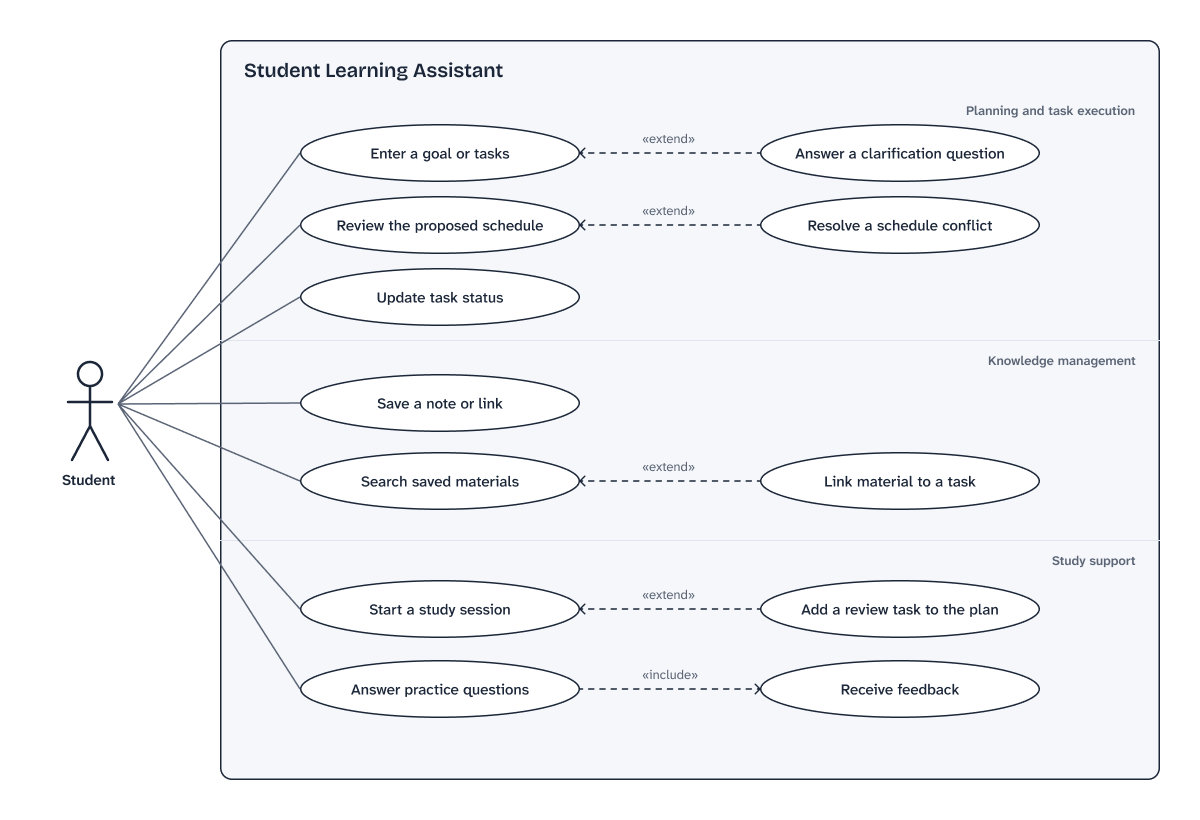
\includegraphics[width=\textwidth]{img/usecase-diagram.png}
\caption{Use case diagram, grouped by feature}
\label{fig:usecase-detail}
\end{figure}

\section{Use case specification: plan study tasks}\label{sec:use-case-specification}

\begin{center}
\begin{tabularx}{\textwidth}{|>{\bfseries\raggedright\arraybackslash}p{3.4cm}|X|}
\hline
ID and name & UC-01, Plan and track study tasks. \\ \hline
Primary actor & Student. \\ \hline
Goal & Turn a goal or task list into structured tasks and a schedule proposal that the student can review and edit. \\ \hline
Preconditions & The student has a goal or at least one task to plan, and the system can accept input. A personal calendar connection is not required. \\ \hline
Trigger & The student opens the planning feature and enters a goal, tasks, or a request to change the current plan. \\ \hline
Postconditions & The system displays structured tasks, a proposed schedule when sufficient information is available, assumptions or warnings, and task statuses. The student can accept, edit, or recalculate the proposal. \\ \hline
\end{tabularx}
\end{center}

\subsection*{Main flow}
\begin{enumerate}
  \item The student enters a goal or describes the work. They may include deadlines, durations, priorities, dependencies, and available time.
  \item The system extracts identifiable facts, breaks the goal into tasks, and marks details that are missing.
  \item The system presents a draft task list for review and distinguishes extracted facts from suggestions.
  \item If the required information is available, the system orders tasks by dependencies and priority, then checks durations against availability and deadlines.
  \item The system produces a proposed schedule, lists conflicts or unscheduled tasks, and explains the relevant constraints.
  \item The student reviews the result, edits details, or updates task status.
  \item When something changes, the system updates the plan and presents the revised proposal for the student to review.
\end{enumerate}

\subsection*{Alternative and exception flows}
\begin{enumerate}
  \item \textbf{A1, Missing information:} If a detail needed for scheduling is missing, such as duration or availability, the system asks a focused question. After the student responds, the flow resumes at step 2. If they skip the question, the system can keep the task list and explain why it cannot schedule the work yet.
  \item \textbf{A2, Conflict or infeasible schedule:} The system identifies the conflict and lists work it could not schedule. It asks the student to revise the constraints instead of presenting the result as feasible.
  \item \textbf{A3, Student edits the result:} If the student changes a priority, deadline, or status, the system preserves unchanged facts, updates the affected details, and recalculates the proposal.
  \item \textbf{A4, Unsupported request:} The system explains which part it does not support and does not invent data to complete the request.
\end{enumerate}

Figure~\ref{fig:chat-ui} shows a proposed chat screen for this use case. The assistant highlights the facts it extracted from the student's request and asks for the missing study hours (A1). The draft schedule then reports that the midterm review does not fit before the deadline (A2). The plan panel separates facts the student supplied from estimates the system assumed.

\begin{figure}[H]
\centering
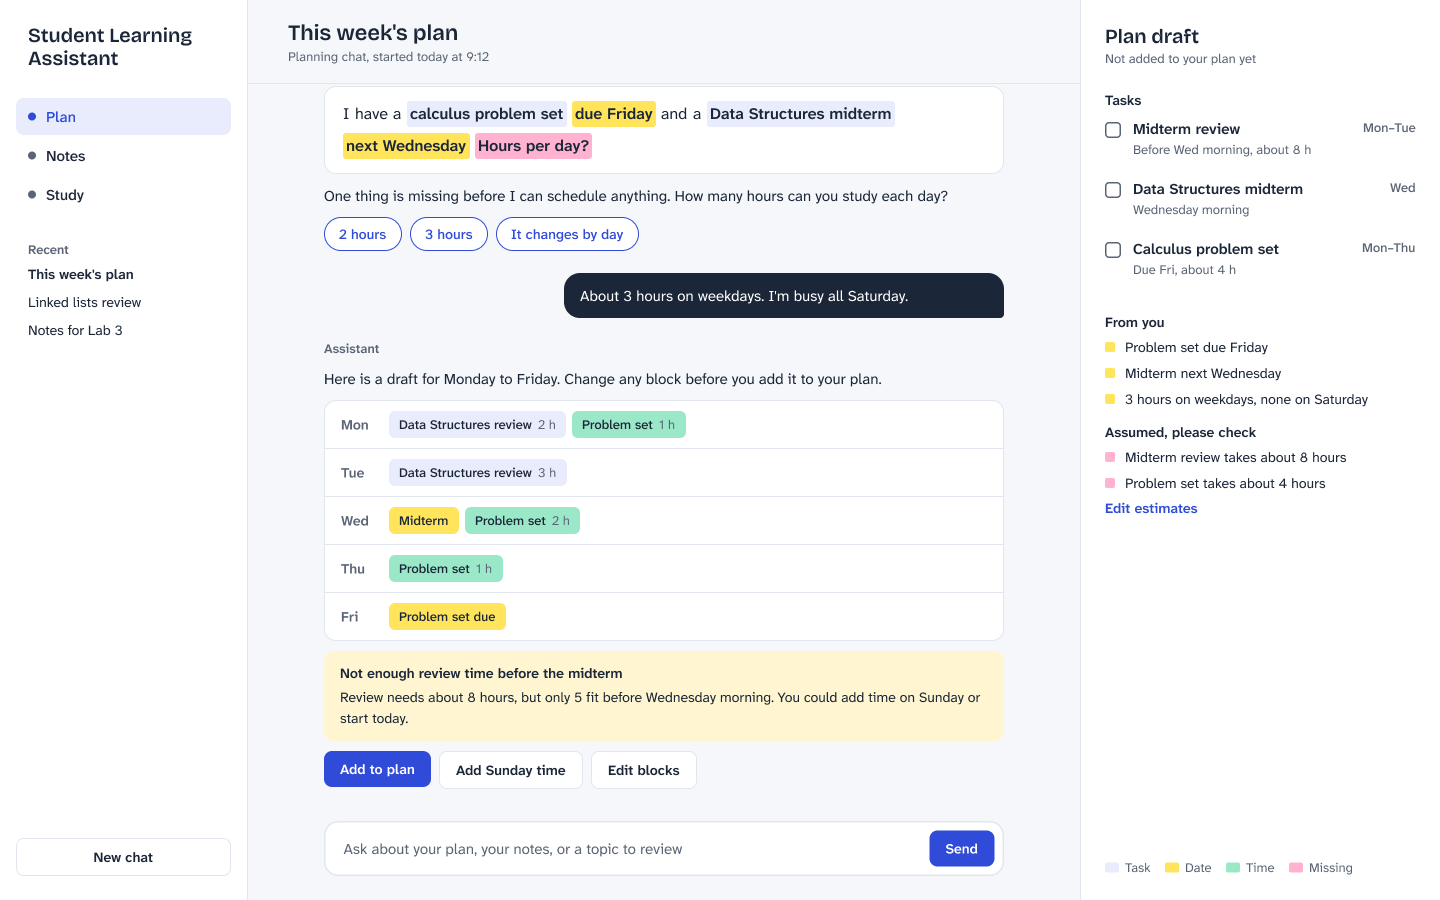
\includegraphics[width=\textwidth]{img/chat-ui.png}
\caption{Proposed chat screen for planning study tasks}
\label{fig:chat-ui}
\end{figure}

\section{Conceptual data model}

The team proposes an \texttt{AssistantContext} for each learning session or context. It references the entities below so the three features can share information while keeping separate responsibilities. The context does not decide what a student should value or prioritize. Each entity below maps to one table in the proposed database.

\begin{longtable}{|>{\raggedright\arraybackslash}p{3.5cm}|>{\raggedright\arraybackslash}p{6.0cm}|>{\raggedright\arraybackslash}p{5.5cm}|}
\hline
\textbf{Entity} & \textbf{Proposed core attributes} & \textbf{Purpose and relationships} \\ \hline
\endhead
AssistantContext & context\_id, user\_goal, next\_actions, created\_at & Shared context linking goals with tasks, knowledge items, and study sessions. \\ \hline
Task & task\_id, context\_id, title, deadline?, duration\_min?, priority?, status, source & A unit of work. The source field records whether the student supplied it or the system suggested it. \\ \hline
ScheduleBlock & block\_id, task\_id, start\_at, end\_at, status, assumption? & A proposed time slot for a task. Some tasks may remain unscheduled. \\ \hline
TaskDependency & task\_id, depends\_on\_id & Records that one task cannot start before another task is finished. \\ \hline
KnowledgeItem & item\_id, context\_id, title, content\_ref, source\_url?, tags, created\_at & User-provided material linked to a goal or task. \\ \hline
TaskKnowledge & task\_id, item\_id & Links a task to the materials it uses. \\ \hline
StudySession & session\_id, context\_id, topic, progress, review\_notes, started\_at & A learning session whose result can create a next action or review task. \\ \hline
StudySessionItem & session\_id, item\_id & Links a study session to the materials it covers. \\ \hline
\end{longtable}

A question mark marks an attribute that may be unknown. During implementation, the team will need to decide how to represent dates and time zones, validate input, and handle edits or deletions to linked records. The proposal does not select a database technology. Figure~\ref{fig:database} shows these tables with their primary and foreign keys. Task dependencies and the links between materials and tasks or study sessions are many-to-many relationships, so each is stored in its own linking table: TaskDependency, TaskKnowledge, and StudySessionItem.

\begin{figure}[H]
\centering
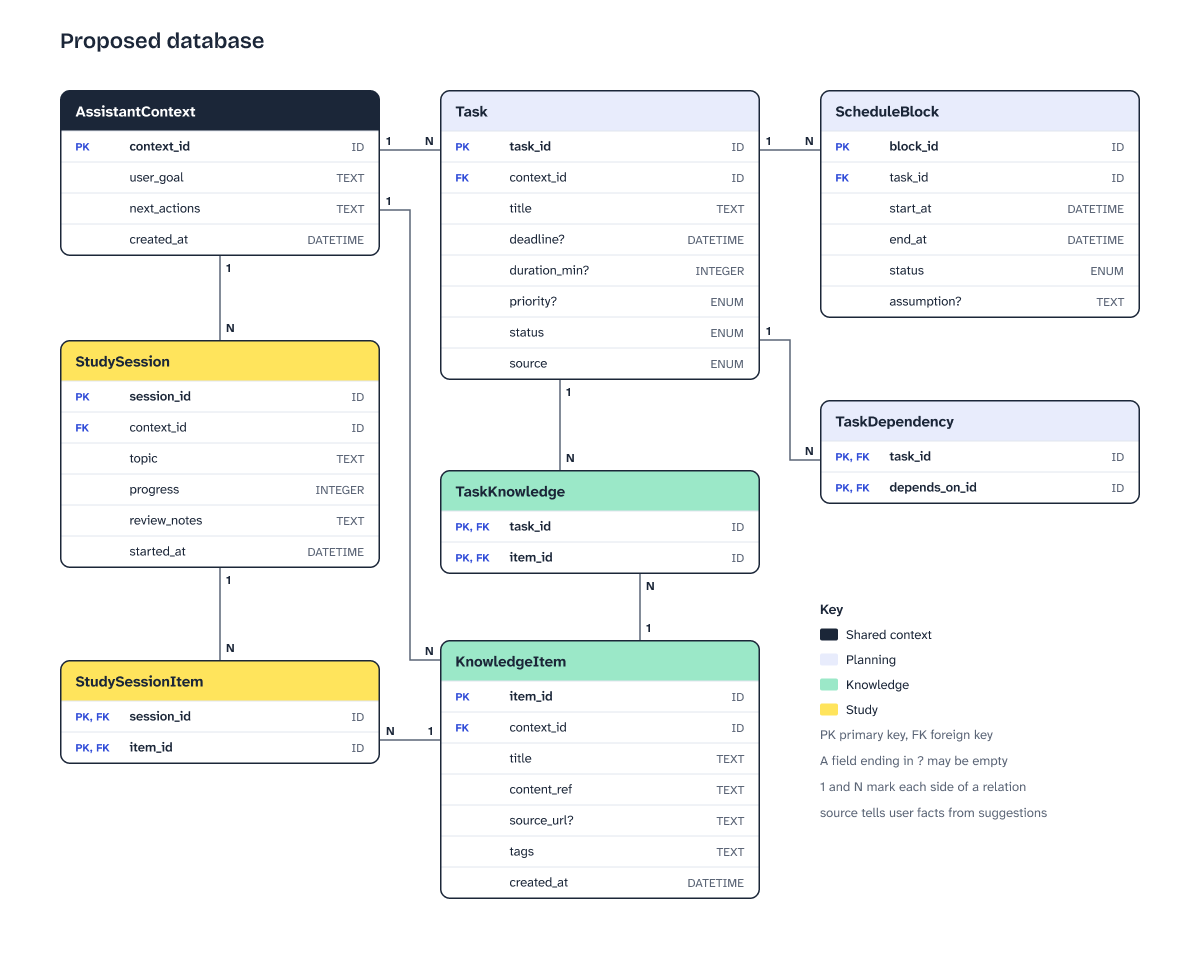
\includegraphics[width=\textwidth]{img/database-diagram.png}
\caption{Proposed database diagram}
\label{fig:database}
\end{figure}

\section{Computational thinking in the requirements}

\begin{itemize}
  \item \textbf{Decomposition:} Divide the problem into three features with separate inputs, processes, and outputs. Break planning into fact extraction, clarification, task management, constraint checking, scheduling, and progress tracking.
  \item \textbf{Pattern recognition:} Reuse workflows such as goal, action, progress check, and revision; capture, organize, retrieve, and connect; explain, practise, give feedback, and review.
  \item \textbf{Abstraction:} Keep details that affect study work, such as goals, tasks, deadlines, materials, and status. Ignore presentation details such as interface colour or device type when they do not affect processing. Use a shared context to connect entities without merging feature responsibilities.
  \item \textbf{Algorithm design:} Check for missing details before scheduling, respect stated dependencies and constraints, and report conflicts or unscheduled tasks. The team will refine and test the priority and scheduling rules with synthetic data.
\end{itemize}

\subsection*{Proposed scheduling workflow}
\begin{enumerate}
  \item Extract tasks and facts supplied by the student.
  \item Mark required details that are missing or inconsistent. Ask the student to clarify and pause scheduling if needed.
  \item Order tasks by dependency. Within each dependency level, use confirmed deadlines and priorities.
  \item For each task, find an available time slot before its deadline that respects dependencies.
  \item Add a suitable slot to the proposed schedule. If no slot fits, mark the task as unscheduled and record the conflicting constraint.
  \item Present the schedule, assumptions, warnings, and unscheduled tasks for review.
\end{enumerate}

Evaluation should check that a proposed schedule respects the supplied deadlines, durations, availability, and dependencies. Tests should also cover missing details and cases with no feasible schedule.
